\documentclass[12pt,aspectratio=169]{beamer}
\usepackage[UTF8]{ctex}  % 支持中文
\usepackage{tikz}
\usepackage{geometry}
\usepackage{minted}  % 用于源代码高亮显示
\usetikzlibrary{calc} % 用于计算坐标

% 页面尺寸设置
\setbeamersize{text margin left=1cm, text margin right=1cm}
\geometry{paperwidth=240mm, paperheight=135mm}

% 设置主题
\usetheme{Madrid}  % Madrid主题
\usecolortheme{beaver}  % 使用beaver主题颜色

\setminted{
    autogobble=true,         % 自动去除多余空白行
    bgcolor=black!5,         % 设置背景颜色
    fontfamily=tt,           % 字体:默认tt,等宽字体;rm,衬线字体;sf,无衬线字体 
    fontsize=\large,         % 设置字体大小    
    frame=single,            % 设置边框类型
    framesep=5pt,            % 设置边框和代码的间距
    highlightcolor=yellow,   % 高亮颜色
    linenos=true,            % 显示行号
    numberblanklines=true,   % 空行是否显示行号    
    numbersep=5pt,           % 设置行号和代码的间距
    showspaces=false,        % 是否显示空格  
    style=xcode,             % 选择语法高亮风格
    tabsize=2,               % 设置Tab大小    
    xleftmargin=24pt,        % 设置左侧缩进
    xrightmargin=24pt,       % 设置右侧缩进     
}

\begin{document}

\title{LaTeX绘图讲稿}
\author{丁保华}
\institute{致慧星空工作室}
\date{\today}
\frame{\titlepage}

\begin{frame}[fragile]
\frametitle{画点}

% 源代码高亮显示
\begin{minted}[frame=single,framesep=10pt]{latex}
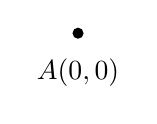
\begin{tikzpicture}
    \fill (0,0) circle (2pt);  % 画一个点,坐标是(0, 0)
    \node at (0,-0.5) {$A(0, 0)$};  % 标注点 A
\end{tikzpicture}
\end{minted}

% 显示画图结果
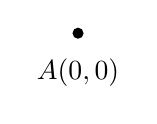
\begin{tikzpicture}
    \fill (0,0) circle (2pt);  % 画一个点,坐标是(0, 0)
    \node at (0,-0.5) {$A(0, 0)$};  % 标注点 A
\end{tikzpicture}

\end{frame}

\begin{frame}[fragile]
\frametitle{画线段}

% 源代码高亮显示
\begin{minted}[frame=single,framesep=10pt]{latex}
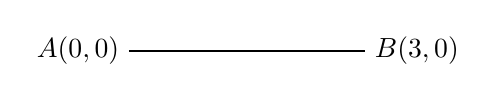
\begin{tikzpicture}
    \draw[thick] (0,0) -- (3,0);  % 画一条从(0,0)到(3,0)的线段
    \node at (0,0) [left] {$A(0,0)$}; % 标注点A
    \node at (3,0) [right] {$B(3,0)$};  % 标注点B
\end{tikzpicture}
\end{minted}

% 显示画图结果
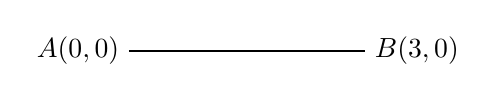
\begin{tikzpicture}
    \draw[thick] (0,0) -- (3,0);  % 画一条从(0,0)到(3,0)的线段
    \node at (0,0) [left] {$A(0,0)$}; % 标注点A
    \node at (3,0) [right] {$B(3,0)$};  % 标注点B
\end{tikzpicture}

\end{frame}

\begin{frame}[fragile]
\frametitle{画三角形}

% 源代码高亮显示
\begin{minted}[frame=single,framesep=10pt]{latex}
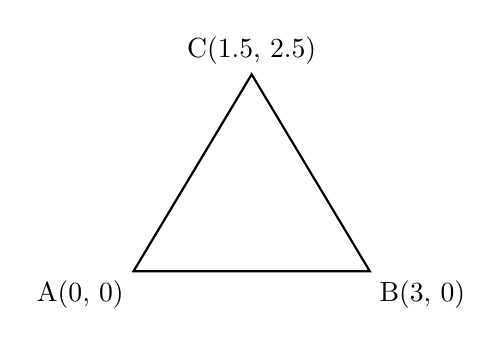
\begin{tikzpicture}
    \draw[thick] (0,0) -- (3,0) -- (1.5,2.5) -- cycle;  % 画一个三角形
    \node at (0,0) [below left] {A(0, 0)}; % 标注点A
    \node at (3,0) [below right] {B(3, 0)}; % 标注点B
    \node at (1.5,2.5) [above] {C(1.5, 2.5)}; % 标注点C
\end{tikzpicture}
\end{minted}

% 显示画图结果
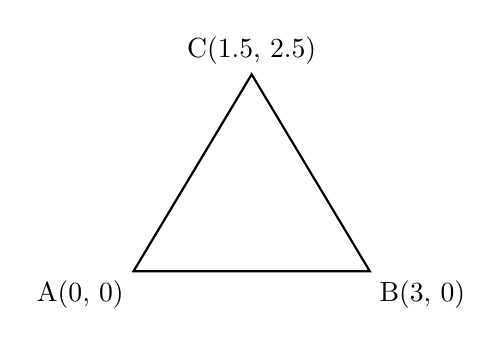
\begin{tikzpicture}
    \draw[thick] (0,0) -- (3,0) -- (1.5,2.5) -- cycle;  % 画一个三角形
    \node at (0,0) [below left] {A(0, 0)}; % 标注点A
    \node at (3,0) [below right] {B(3, 0)}; % 标注点B
    \node at (1.5,2.5) [above] {C(1.5, 2.5)}; % 标注点C
\end{tikzpicture}

\end{frame}

\begin{frame}[fragile]
\frametitle{画长方形}

% 源代码高亮显示
\begin{minted}[frame=single,framesep=10pt]{latex}
\begin{tikzpicture}
    \draw[thick] (0,0) rectangle (4,2);  % 画一个长方形
    \node at (0,-0.5)  [below left] {$A(0, 0)$}; % 标注点A
    \node at (4,-0.5) [below right] {$B(4, 0)$}; % 标注点B
    \node at (4,2.5) [above right] {$C(4, 2)$}; % 标注点C
    \node at (0,2.5) [above left] {$D(0, 2)$}; % 标注点D
\end{tikzpicture}
\end{minted}

% 显示画图结果
\begin{tikzpicture}
    \draw[thick] (0,0) rectangle (4,2);  % 画一个长方形
    \draw[thick] (0,0) rectangle (4,2);  % 画一个长方形
    \node at (0,-0.5)  [below left] {$A(0, 0)$}; % 标注点A
    \node at (4,-0.5) [below right] {$B(4, 0)$}; % 标注点B
    \node at (4,2.5) [above right] {$C(4, 2)$}; % 标注点C
    \node at (0,2.5) [above left] {$D(0, 2)$}; % 标注点D
\end{tikzpicture}

\end{frame}

\begin{frame}[fragile]
\frametitle{画圆}

% 源代码高亮显示
\begin{minted}[frame=single,framesep=10pt]{latex}
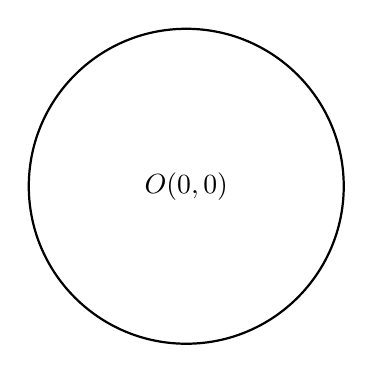
\begin{tikzpicture}
    \draw[thick] (0,0) circle(2);  % 画一个圆,圆心(0, 0),半径2
    \node at (0,0) {$O(0, 0)$}; % 标注圆心
\end{tikzpicture}
\end{minted}

% 显示画图结果
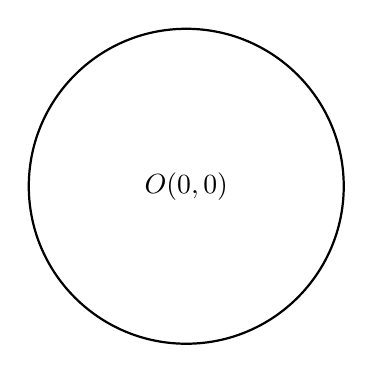
\begin{tikzpicture}
    \draw[thick] (0,0) circle(2);  % 画一个圆,圆心(0, 0),半径2
    \node at (0,0) {$O(0, 0)$}; % 标注圆心
\end{tikzpicture}

\end{frame}

\begin{frame}[fragile]
\frametitle{画椭圆}

% 源代码高亮显示
\begin{minted}[frame=single,framesep=10pt]{latex}
\begin{tikzpicture}
    \draw[thick] (0,0) ellipse(3 and 2);  % 画一个椭圆,半长轴3,半短轴2
    \node at (0,-2.5) {椭圆中心 O(0, 0)};
\end{tikzpicture}
\end{minted}

% 显示画图结果
\begin{tikzpicture}
    \draw[thick] (0,0) ellipse(3 and 2);  % 画一个椭圆,半长轴3,半短轴2
    \node at (0,-2.5) {椭圆中心 O(0, 0)};
\end{tikzpicture}

\end{frame}

\begin{frame}[fragile]
\frametitle{画圆弧--文档有错误}

% 源代码高亮显示
\begin{minted}[frame=single,framesep=10pt]{latex}
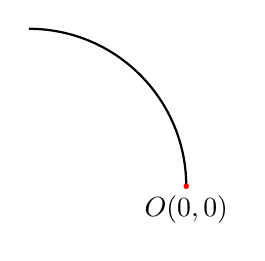
\begin{tikzpicture}
    \draw[thick] (0,0) arc[start angle=0, end angle=90, radius=2];  % 画一个圆弧
    \node at (0,0) [below ]{$O(0,0)$}; % 标注圆心
    \fill (0,0) [red] circle(1pt);

\end{tikzpicture}
\end{minted}

% 显示画图结果
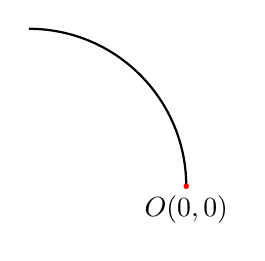
\begin{tikzpicture}
    \draw[thick] (0,0) arc[start angle=0, end angle=90, radius=2];  % 画一个圆弧
    \node at (0,0) [below ]{$O(0,0)$}; % 标注圆心
    \fill (0,0) [red] circle(1pt);

\end{tikzpicture}

\end{frame}

\begin{frame}[fragile]
\frametitle{画圆弧--正确的代码}

% 源代码高亮显示
\begin{minted}[frame=single,framesep=10pt]{latex}
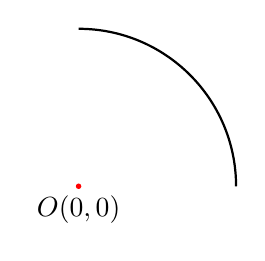
\begin{tikzpicture}
    \draw[thick] (0,0)+(2,0) arc[start angle=0, end angle=90, radius=2];  % 画一个圆弧
    \node at (0,0) [below ]{$O(0,0)$}; % 标注圆心
    \fill (0,0) [red] circle(1pt);

\end{tikzpicture}
\end{minted}

% 显示画图结果
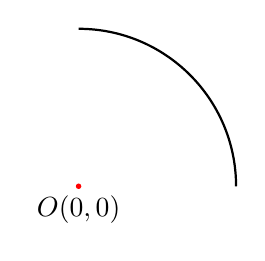
\begin{tikzpicture}
    \draw[thick] (0,0)+(2,0) arc[start angle=0, end angle=90, radius=2];  % 画一个圆弧
    \node at (0,0) [below ]{$O(0,0)$}; % 标注圆心
    \fill (0,0) [red] circle(1pt);

\end{tikzpicture}

\end{frame}

\begin{frame}[fragile]
\frametitle{画圆弧--使用极坐标系}

% 源代码高亮显示
\begin{minted}[frame=single,framesep=10pt]{latex}
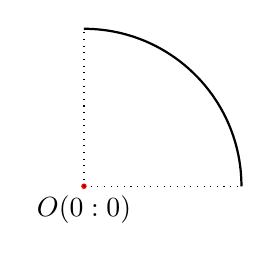
\begin{tikzpicture}
    \draw[thick] (0:2) arc(0:90:2);  % 画一个圆弧,0度角到90度角,半径2
    \node at (0:0) [below ]{$O(0:0)$}; % 标注圆心
    \fill (0:0) [red] circle(1pt);
    \draw [dotted] (0:0) -- (0:2); % 用点线连接原点与圆弧起点
    \draw [dotted] (0:0) -- (90:2);  % 用点线连接原点与圆弧终点

\end{tikzpicture}
\end{minted}

% 显示画图结果
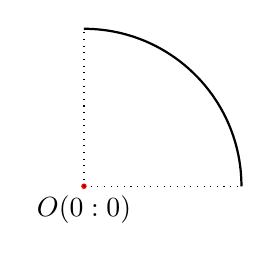
\begin{tikzpicture}
    \draw[thick] (0:2) arc(0:90:2);  % 画一个圆弧,0度角到90度角,半径2
    \node at (0:0) [below ]{$O(0:0)$}; % 标注圆心
    \fill (0:0) [red] circle(1pt);
    \draw [dotted] (0:0) -- (0:2); % 用点线连接原点与圆弧起点
    \draw [dotted] (0:0) -- (90:2);  % 用点线连接原点与圆弧终点
    
\end{tikzpicture}

\end{frame}


\end{document}
